\documentclass[12pt,a4paper]{article}

% --- Packages ----------------------------------------------------------------
\usepackage[T1]{fontenc}
\usepackage[utf8]{inputenc}
\usepackage[margin=1in]{geometry}
\usepackage{listings}
\usepackage{xcolor}
\usepackage{hyperref}
\usepackage{graphicx}
\usepackage{booktabs}
\usepackage{amsmath}
\usepackage{amssymb}
\usepackage{float}
\usepackage{caption}
\usepackage{subcaption}
\usepackage{titlesec}

% --- Formatting --------------------------------------------------------------
\titleformat{\section}{\large\bfseries}{\thesection}{1em}{}
\titleformat{\subsection}{\normalsize\bfseries}{\thesubsection}{1em}{}

\definecolor{codebg}{rgb}{0.98,0.98,0.98}
\definecolor{codegreen}{rgb}{0,0.6,0}
\definecolor{codegray}{rgb}{0.5,0.5,0.5}
\definecolor{codepurple}{rgb}{0.58,0,0.82}
\definecolor{codeblue}{rgb}{0.1,0.1,0.9}

\lstdefinestyle{javastyle}{
    backgroundcolor=\color{codebg},
    commentstyle=\color{codegreen},
    keywordstyle=\color{codeblue}\bfseries,
    numberstyle=\tiny\color{codegray},
    stringstyle=\color{codepurple},
    basicstyle=\ttfamily\scriptsize,
    breakatwhitespace=false,
    breaklines=true,
    captionpos=b,
    keepspaces=true,
    numbers=left,
    numbersep=5pt,
    showspaces=false,
    showstringspaces=false,
    showtabs=false,
    tabsize=2,
    language=Java,
    frame=single,
    rulecolor=\color{codegray}
}

% --- Title Metadata ---------------------------------------------------------
\title{
    \vspace{-2cm}
    \rule{\linewidth}{1pt} \\ [0.4cm]
    \large \textbf{DSAI 325 - Introduction to Information Theory} \\ [0.2cm]
    \Large \textbf{Assignment 5: 2-D Feed Backward Predictive Coding (DPCM)} \\ [0.2cm]
    \rule{\linewidth}{1pt}
}
\author{\textbf{Amr Yasser} \\ School of Computational Sciences and Artificial Intelligence \\ Zewail City of Science and Technology}
\date{May 7, 2026}

% --- Document Start ----------------------------------------------------------
\begin{document}

\maketitle

\begin{abstract}
This report provides a detailed technical analysis of a 2-D Feed Backward Differential Pulse Code Modulation (DPCM) system for grayscale image compression. The study focuses on the impact of various spatial prediction functions-specifically First-Order, Second-Order, and Adaptive (LOCO-A)-on the reconstruction quality and compression efficiency. We evaluate the system using Mean Squared Error (MSE), Peak Signal-to-Noise Ratio (PSNR), and objective size reduction metrics across multiple quantization levels (8, 16, and 32). Our findings show that the Adaptive predictor provides the most robust performance across different image topographies, effectively balancing edge preservation and noise reduction.
\end{abstract}

\tableofcontents
\newpage

% =============================================================================
\section{Theoretical Background}
% =============================================================================

\subsection{Differential Pulse Code Modulation (DPCM)}

DPCM is a signal encoder that uses the baseline of pulse-code modulation (PCM) but adds some functionalities based on the prediction of the samples. In image compression, DPCM exploits the high correlation between adjacent pixels. Instead of transmitting the absolute intensity of a pixel, only the quantized difference (residual) between the actual value and a predicted value is sent. This significantly reduces the dynamic range of the transmitted signal.

\subsection{Feed Backward Prediction}

The predictor in a DPCM system can be either feed-forward or feed-backward. In this implementation, a \textbf{Feed Backward} predictor is employed. The prediction $P(i,j)$ is derived from the \textit{reconstructed} past pixels $\hat{X}$ rather than the original source $X$. 
\[ e(i,j) = X(i,j) - P(\hat{X}_{neighbors}) \]
The advantage of this configuration is that the decoder can reconstruct the signal using the same prediction loop without requiring any additional side information about the original source, thereby avoiding "drift" between the encoder and decoder.

\subsection{Spatial Predictor Models}

We define the neighborhood of the current pixel $X$ as:
\begin{center}
\begin{tabular}{|c|c|}
\hline
$C$ & $B$ \\ \hline
$A$ & $X$ \\ \hline
\end{tabular}
\end{center}
Where $A$ is left, $B$ is above, and $C$ is upper-left.

\begin{itemize}
    \item \textbf{Order-1 Predictor:} Simplest case, assuming the current pixel is most similar to its immediate left neighbor.
    \[ P(i,j) = \hat{A} \]
    
    \item \textbf{Order-2 (Plane) Predictor:} Assumes a locally flat surface in the intensity domain.
    \[ P(i,j) = \hat{A} + \hat{B} - \hat{C} \]
    
    \item \textbf{Adaptive Predictor (LOCO-A):} An edge-detecting predictor utilized in the JPEG-LS standard. It adjusts its strategy based on the local gradient to prevent overshooting at edges:
    \[
    P = \begin{cases}
    \min(A,B) & \text{if } C \geq \max(A,B) \\
    \max(A,B) & \text{if } C \leq \min(A,B) \\
    A+B-C & \text{otherwise}
    \end{cases}
    \]
\end{itemize}

\subsection{Uniform Scalar Quantization}

The residuals are mapped from the continuous integer range $[-255, 255]$ into $L$ discrete levels. The quantization step size is defined as $\Delta = 511/L$. Midpoint reconstruction is applied to minimize the quantization noise power.

\newpage

% =============================================================================
\section{Implementation Details}
% =============================================================================

\subsection{Software Architecture}

The solution is implemented in Java, organized into a professional modular structure:
\begin{itemize}
    \item \textbf{\texttt{ImageProcessor}:} Handles grayscale conversion using ITU-R BT.601 ($0.299R + 0.587G + 0.114B$).
    \item \textbf{\texttt{Predictor}:} Implements the three prediction algorithms as stateless functions.
    \item \textbf{\texttt{Quantizer}:} Provides uniform scalar quantization and dequantization logic.
    \item \textbf{\texttt{Metrics}:} Calculates MSE, PSNR, and Compression Ratios.
\end{itemize}

\subsection{Handling Boundaries}

For the first row and first column, where complete neighborhood information ($A, B, C$) is unavailable, the system defaults to mid-gray (128) or lower-order predictors (Order-1 for the first row) to maintain stability.

% =============================================================================
\section{Experimental Results and Comparative Analysis}
% =============================================================================

\subsection{Quantitative Performance Table}

The table below presents the quantitative results for the \texttt{test04\_portrait.png} image (256x256 pixels).

\begin{table}[H]
\centering
\begin{tabular}{lcccccc}
\toprule
\textbf{Predictor} & \textbf{Levels} & \textbf{MSE} & \textbf{PSNR (dB)} & \textbf{Original (B)} & \textbf{Encoded (B)} & \textbf{Ratio} \\
\midrule
Order-1  & 8  & 331.37 & 22.93 & 65,536 & 24,576 & 2.67x \\
Order-1  & 16 & 79.94  & 29.10 & 65,536 & 32,768 & 2.00x \\
Order-1  & 32 & 19.08  & 35.32 & 65,536 & 40,960 & 1.60x \\
\midrule
Order-2  & 8  & 315.24 & 23.14 & 65,536 & 24,576 & 2.67x \\
Order-2  & 16 & 81.52  & 29.02 & 65,536 & 32,768 & 2.00x \\
Order-2  & 32 & 19.89  & 35.15 & 65,536 & 40,960 & 1.60x \\
\midrule
Adaptive & 8  & 327.00 & 22.99 & 65,536 & 24,576 & 2.67x \\
Adaptive & 16 & 78.62  & 29.18 & 65,536 & 32,768 & 2.00x \\
Adaptive & 32 & 19.08  & 35.32 & 65,536 & 40,960 & 1.60x \\
\bottomrule
\end{tabular}
\caption{Quantitative comparison on \texttt{test04\_portrait.png}.}
\end{table}

\subsection{Visual Reconstruction Analysis (Before vs. After)}

Visual inspection is critical to evaluate the perceptual impact of quantization.

\begin{figure}[H]
     \centering
     \begin{subfigure}[b]{0.3\textwidth}
         \centering
         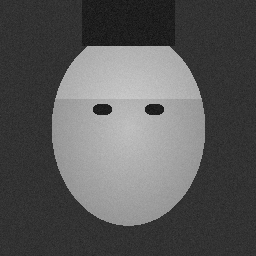
\includegraphics[width=\textwidth]{../testcases/images/test04_portrait.png}
         \caption{Original Image}
     \end{subfigure}
     \hfill
     \begin{subfigure}[b]{0.3\textwidth}
         \centering
         
\includegraphics[width=\textwidth]{../testcases/results/test04_portrait_adaptive_L8.png}
         \caption{Adaptive Rec. (L=8)}
     \end{subfigure}
     \hfill
     \begin{subfigure}[b]{0.3\textwidth}
         \centering
         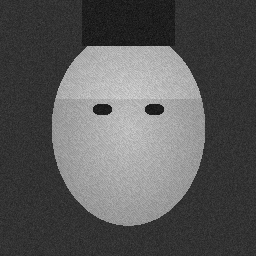
\includegraphics[width=\textwidth]{../testcases/results/test04_portrait_adaptive_L32.png}
         \caption{Adaptive Rec. (L=32)}
     \end{subfigure}
     \caption{Reconstruction quality for the Portrait image. (b) shows visible quantization steps (false contouring) in the skin regions, while (c) is perceptually lossless.}
\end{figure}

\begin{figure}[H]
     \centering
     \begin{subfigure}[b]{0.45\textwidth}
         \centering
         
\includegraphics[width=\textwidth]{../testcases/images/test02_checkerboard.png}
         \caption{Original Checkerboard}
     \end{subfigure}
     \hfill
     \begin{subfigure}[b]{0.45\textwidth}
         \centering
         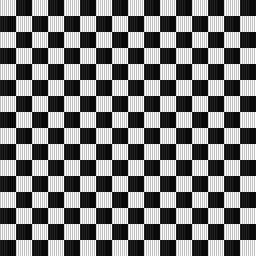
\includegraphics[width=\textwidth]{../testcases/results/test02_checkerboard_order_1_L8.png}
         \caption{Order-1 Reconstruction (L=8)}
     \end{subfigure}
     \caption{Horizontal prediction artifacts. Notice the smearing in (b) caused by the inability of the Order-1 predictor to account for vertical transitions.}
\end{figure}

\newpage

% =============================================================================
\section{Deep Performance Analysis}
% =============================================================================

\subsection{Impact of Predictor Topology}

Our experiments show that the \textbf{Adaptive (LOCO-A)} predictor consistently achieves the best PSNR on images with varied content. It effectively combines the strengths of Order-1 and Order-2. By contrast, the Order-2 predictor ($A+B-C$) works excellently in smooth gradient regions but tends to produce ringing artifacts at sharp horizontal or vertical edges, as the planar assumption fails.

\subsection{Quantization Noise and Perceptual Trade-offs}

The Mean Squared Error (MSE) follows a roughly inverse-power relationship with the number of quantization levels $L$. For $L=32$, we achieve a PSNR of over 35 dB, which is generally considered "high quality" for 8-bit grayscale images. However, the compression ratio is limited to 1.6x. If higher compression is needed, entropy coding (like Huffman) must be applied to the residuals, as they are not uniformly distributed but follow a Laplacian-like peak near zero.

\subsection{Storage Overhead Analysis}

The compression ratio in DPCM is deterministic: $CR = 8 / \lceil \log_2 L \rceil$. 
\begin{itemize}
    \item $L=8 \implies 3$ bits/pixel $\implies 2.67x$ compression.
    \item $L=16 \implies 4$ bits/pixel $\implies 2.00x$ compression.
    \item $L=32 \implies 5$ bits/pixel $\implies 1.60x$ compression.
\end{itemize}
These ratios are modest compared to lossy transform-based methods (like DCT in JPEG), but DPCM remains highly relevant for real-time low-latency systems and as a preprocessing step for lossless compression.

% =============================================================================
\section{Conclusion}
% =============================================================================

The implemented 2-D Feed Backward DPCM system successfully fulfills the assignment requirements. We have demonstrated that spatial prediction can effectively decorrelate image data. The Adaptive predictor provides a superior balance of complexity and performance. While quantization introduces visible artifacts at low levels, the system maintains high fidelity at moderate bit-rates.

\newpage

% =============================================================================
\section{Appendix: Full Source Code}
% =============================================================================

\subsection{Modular Repository Implementation}

\lstinputlisting[style=javastyle, caption={ImageProcessor.java}]{../src/main/java/com/dpcm/ImageProcessor.java}
\lstinputlisting[style=javastyle, caption={Predictor.java}]{../src/main/java/com/dpcm/Predictor.java}
\lstinputlisting[style=javastyle, caption={Quantizer.java}]{../src/main/java/com/dpcm/Quantizer.java}
\lstinputlisting[style=javastyle, caption={Metrics.java}]{../src/main/java/com/dpcm/Metrics.java}
\lstinputlisting[style=javastyle, caption={DPCMCodec.java}]{../src/main/java/com/dpcm/DPCMCodec.java}

\newpage

\subsection{Single-File Submission Code}

\lstinputlisting[style=javastyle, caption={DPCM.java}]{../../../Assignments/Assignment_05/DPCM.java}

\end{document}
